\documentclass[12pt,a4paper]{article}

\usepackage[utf8]{inputenc}
\usepackage{amsmath}
\usepackage{amsfonts}
\usepackage{amssymb}
\usepackage{lmodern}
\usepackage{setspace}
\usepackage{siunitx}
\usepackage[ngerman]{babel}
\usepackage{tikz}
\usetikzlibrary{shapes,arrows,calc}
\usepackage[european]{circuitikz}

\newcommand{\reffig}[1]{{Abb.~\ref{fig:#1}}}
\newcommand{\reftab}[1]{{Tab.~\ref{tab:#1}}}
\newcommand{\refeq}[1]{{(\ref{eq:#1})}}
\newcommand{\refsec}[1]{{Abschnitt~\ref{sec:#1}}}
 
\author{Benedikt Schmidt}
\title{Validierung von \emph{Holomorphic Embedding Load Flow}}

\hyphenation{Ge-nau-ig-keit}

\begin{document}
	\maketitle
	\newpage
	\tableofcontents
	\newpage
	
	\section{Einführung}
	Klassische Verfahren zur Berechnung von Lastflüssen in elektrischen Energieverteilungsnetzen, wie zum Beispiel die \emph{Stromiteration} oder \emph{Fast-de\-cou\-pled-load-flow} (\emph{FDLF}), weisen erhebliche Probleme in Bezug auf die Konvergenz auf. Zum einen können diese iterative Verfahren unter Umständen gar nicht konvergieren, obwohl das zu berechnende System an sich stabil wäre. Zusätzlich dazu können die berechneten Lösungen in bestimmten Situationen keine physikalische Lösung des Systems beschreiben. \emph{Holomorphic embedding load flow} (\emph{HELM}) \cite{helmIEEE}, ein von \emph{Antonio Trias} neu entwickelter Ansatz zur Lastflussberechnung, verspricht diese Probleme zu lösen. Die praktische Valdidierung dieser Aussagen erfolgte von mir durch die Entwicklung eines Programmes, welches sowohl \emph{HELM} als auch die klassischen iterativen Verfahren implementiert.
	
	\section{Berechnung der Knotenspannungen in \emph{HELM}}
	Ausgangsproblem ist ein elektrisches Energieverteilungsnetz bestehend aus Knoten bzw. sogenannten Bussen und Admittanzen $Y_{ij}$, welche die Knoten verbinden. Zudem muss an mindestens einem Knoten, dem Slackbus, Real- und Imaginärteil der Spannung zur Definition des Winkels vorgegeben sein. An allen anderen Knoten müssen dann jeweils genau zwei der folgenden Größen vorgegeben sein: $P_i$, $Q_i$, $\Re\{U_i\}$, $\Im\{U_i\}$ oder $|U_i|$. Bei einer Vorgabe von $|U_i|$ und $P_i$ spricht man von einem PV-Bus, bei $P_i$ und $Q_i$ von einem PQ-Bus. Im folgenden werde ich mich immer auf den Fall eines PQ-Busses beziehen, die Modellierung eines PV-Busses in \emph{HELM} wird in \cite{helmPV} behandelt. Die im weiteren Verlauf angeführten Formeln und Methoden entstammen größtenteils \cite{helmIEEE}, \cite{helmPatentApr2009} und \cite{helmPatentSept2009}.
	
	Für einen PQ-Bus ergibt sich aus der Kirchhoffschen Knotenregel
	\begin{equation}
		\sum_j Y_{ij} U_{j} = I_j + \frac{S_j^\star}{U_j^\star},
		\label{eq:loadflow}
	\end{equation}
	wobei die konstanten Ströme $I_j$ der Reduktion des Gesamtsystems um die Slackbusse entstammen.
	
	Die explizite Lösung von \refeq{loadflow} ist an dieser Stelle aufgrund der quadratischen Form, gemischt mit der Konjugation der Knotenspannungen, nicht möglich. Aus diesem Grund heraus wird in \cite{helmPatentSept2009} eine Betrachtung der Spannungen als komplexe Funktionen in einem neuen Parameter $s$ vorgeschlagen. Um zudem zu erreichen, dass diese Funktionen holomporph sind, wird \refeq{loadflow} zu 
	\begin{equation}
		\sum_j Y_{ij} U_{j}(s) = s I_j + \frac{s S_j^\star}{U_j^\star} + (1 - s) \sum_j Y_{ij}
		\label{eq:loadflowEmbedded}
	\end{equation}
	erweitert. Eine Auswertung dieser Gleichung an der Stelle $s = 1$ ergibt wiederum \refeq{loadflow}, womit also über $U_i(s = 1)$ die eigentliche Knotenspannung $U_i$ berechnet werden kann. Das Ziel ist somit nicht mehr direkt die Berechnung von $U_i$, sondern anstelle dessen die Darstellung von $U_i(s)$. Um dies zu erreichen wird $U_i(s)$ durch die reduzierte Laurentreihe 
	\begin{equation}
		U_i(s) = \sum_{n = 0}^\infty c_{i,n} s^n
		\label{eq:powerSeries}
	\end{equation}
	in \refeq{loadflowEmbedded} ersetzt. Damit lassen sich dann durch einen Koeffizientenvergleich Formeln für die sukzessive Berechnung von $c_{i,n}$ ermitteln.
	
	Die direkte Auswertung von \refeq{powerSeries} ist an diesem Punkt meist nicht möglich, da die Reihe an der Stelle 0 entwickelt wurde und der Konvergenzradius in den meisten Fällen erheblich kleiner als 1 ist. Dieses Problem lässt sich allerdings über eine Methode zur analytischen Fortsetzung lösen, zum Beispiel mithilfe des Epsilon Algorithmuses von Wynn \cite{epsilonWynn}.
	
	Theoretisch lässt sich nun für die Lösung nachweisen, dass sie genau dann konvergiert wenn das System stabil ist, also kein Spannungszusammenbruch eintritt. Somit erhält man also an und für sich genau jenes Ergebnis, welches man sich wünscht: Wenn im System die Spannung zusammenbricht konvergiert das Verfahren nicht, falls das System stabil ist konvergiert das Verfahren. Praktisch ist man allerdings nicht in der Lage zum einen beliebig viele Koeffizienten zu berechnen, und zum anderen stößt man an die Grenzen der Rechengenauigkeit. Bereits für sehr einfache Systeme erreichen die Koeffizienten $c_{i,50}$ dermaßen große Werte, dass mit einem 64 Bit Gleitkommadatentyp die Rechenfehler größer als etwaige Verbesserungen in der Genauigkeit des Ergebnisses sind. Auf Ansätze um dieses Problem anzugehen werde ich im nächsten Abschnitt eingehen.
	
	\section{Implementierung}
	\label{sec:implementierung}
	
	Um \emph{HELM}, bzw. genauer gesagt meine Implementierung von \emph{HELM}, mit den klassischen Ansätzen zur Lastflussberechung vergleichen zu können habe ich folgende Berechnungsverfahren implementiert:
	\begin{enumerate}
		\item \emph{Knotenpunktpotentialverfahren}
		\item \emph{Stromiteration}
		\item \emph{Newton-Raphson} (ohne Vereinfachung)
		\item \emph{FDLF}
		\item \emph{HELM} mit doppelter Genauigkeit (64 Bit)
		\item \emph{HELM} mit beliebiger Genauigkeit
		\item \emph{HELM} kombiniert mit \emph{Newton-Raphson}
		\item \emph{HELM} kombiniert mit einer \emph{Stromiteration}
	\end{enumerate}
	
	Die zwei unterschiedlichen Varianten von \emph{HELM} ergeben sich aus der Einschränkung eines 64 Bit Gleitkommadatentyps, in den meisten Programmiersprachen bekannt als double. Da für eine größere Genauigkeit mehr als nur 50 Koeffizienten und somit auch eine größerer Datentyp nötig ist, habe ich diesen Teil, als einzigen, in \emph{C++} entwickelt. Dadurch konnte ich auf Templates zurückgreifen um beliebige Datentypen und darauf basierend Matrizen zu verwenden. Für den Gleitkommadatentyp mit beliebiger Genauigkeit kam \emph{MPIR} \footnote{http://www.mpir.org/} zum Einsatz, für die Template-Matrizenrechnung \emph{Eigen} \footnote{http://eigen.tuxfamily.org/index.php}. Somit sind die einzigen Einschränkungen für die Rechengenauigkeit der verfügbare Arbeitspeicher und die Berechnungsdauer. Insbesondere letztere wird stark verschlechtert durch die Wahl eines größeren Datentyps, dementsprechend ist dieses Berechnungsverfahren vermutlich eher für akademische Zwecke sinnvoll.
	
	Praktisch durchaus nützlich sein könnten die beiden letzten implementierten Berechnungsverfahren in denen jeweils \emph{HELM} mit doppelter Genaugikeit mit einem iterativen Verfahren kombiniert wird. Bei diesen Kombinationen wird zuerst das iterative Verfahren angewandt, da dieses in der Regel um Größenordnungen schneller ist als \emph{HELM}. Falls allerdings das iterative Verfahren nicht konvergiert kommt \emph{HELM} mit doppelter Genauigkeit zum Einsatz und liefert bessere Startwerte, basierend auf denen wiederum das iterative Verfahren angewandt wird. Somit erhält man gewissermaßen die Vorteile beider Welten, die Geschwindigkeit der iterativen Verfahren kombiniert mit der verbesserten Konvergenz bei Situationen nahe dem Spannungszusammenbruch.
	
	\begin{figure}
		\centering
		\begin{tikzpicture}
	\tikzstyle{block} = [
	rectangle, draw, fill=blue!20,
	text width=10em, text centered,
	rounded corners, minimum height=3em,
	node distance=2cm]
	\tikzstyle{cloud} = [draw, ellipse,fill=green!20, node distance=5cm, minimum height=2em]	
	\tikzstyle{lineOneWay} = [draw, ->, >=stealth', thick]
	\tikzstyle{lineTwoWay} = [draw, <->, >=stealth', thick]
	
	\node [block] (databaseUI) {DatabaseUI};
	\node [block, below of=databaseUI] (database) {Database};
	\node [block, below of=database] (calculation) {Calculation};
	\node [block, below of=calculation] (HELM) {HELM};	
	\node [cloud, right of=database] (sqlDatabase) {SQL Server};
	
	\path [lineOneWay] ($(databaseUI.south)$) -- ($(database.north)$);
	\path [lineOneWay] ($(database.south)$) -- ($(calculation.north)$);
	\path [lineOneWay] ($(calculation.south)$) -- ($(HELM.north)$);
	\path [lineTwoWay] ($(database.east)$) -- ($(sqlDatabase.west)$);
\end{tikzpicture}
		\caption{Software Architektur}
		\label{fig:software_architecture}
	\end{figure}
	
	Die Software gliedert sich in mehrere Klassenbibliotheken, welche hierarchisch aufeinander aufbauen. Die wichtigsten Teile zusammengefasst finden sich in \reffig{software_architecture}. Die Implementierung von \emph{HELM} ist dabei als einziger Teil in \emph{C++}, der Rest ist in \emph{C\#} implementiert. Außerdem gibt es für die meisten Bibliotheken ein Pendant mit Unittests, welche mit Hilfe des in \emph{Visual Studio} integrierten Testframeworks ausgeführt werden können.
	
	\subsection{Datenbank}
	Im Hintergrund zur eigentlichen Anwendung ist es nötig einen Datenbankserver zu betreiben, idealerweise eine \emph{Microsoft SQL Server} oder \emph{Microsoft SQL Server Express}. Die Informationen über das Netz, also die Tabellen powernets, nodes, loads, transformers, lines, generators und feedins, werden beim Verbinden mit der Datenbank eingelesen. Dementsprechend ist es möglich ohne Verwendung der grafischen Oberfläche direkt über die Datenbank Netze zu definieren. Das dafür zu beachtende Datenbankschema ist in \reffig{database_schema} dargestellt. Die Auswahl des Berechnungsverfahrens erfolgt über die Spalte CalculatorSelection in powernets, die jeweilige Bedeutung der Werte kann \reftab{calculator_selection} entnommen werden.
	
	\begin{table}
		\centering
		\begin{tabular}{c|l}
			CalculatorSelection & Berechnungsverfahren \\ \hline
			0 & \emph{Knotenpunktpotentialverfahren} \\
	        1 & \emph{Stromiteration} \\
	        2 & \emph{Newton-Raphson} \\
	        3 & \emph{FDLF} \\
	        4 & \emph{HELM}, 64 Bit \\
	        5 & \emph{HELM}, 200 Bit \\
	        6 & \emph{HELM} mit \emph{Stromiteration} \\
	        7 & \emph{HELM} mit \emph{Newton-Raphson}
		\end{tabular}
		\caption{Bedeutung der Werte für CalculatorSelection}
		\label{tab:calculator_selection}
	\end{table}
	
	Die Tabellen admittances, admittancenodenames und admittancevalues werden nicht eingelesen und dienen nur der Speicherung der Admittanzmatrix, falls der Benutzer dies wünscht. Sowohl in diesen Tabellen als auch in jenen, in denen die Netze abgebildet werden, sind sämtliche Größen in SI-Einheiten.
	
	\begin{figure}
		\centering
		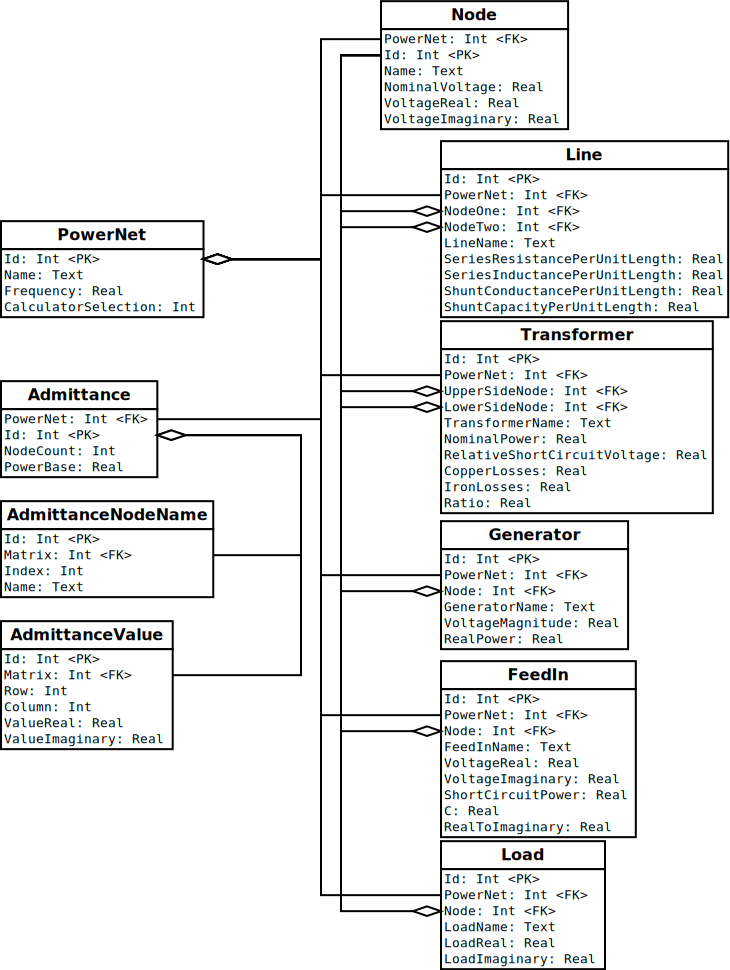
\includegraphics[scale=0.35]{pictures/database_schema}
		\caption{Datenbankschema}
		\label{fig:database_schema}
	\end{figure}
	
	\subsection{Bedienung}
	Zum Start der Anwendung muss die Datei \emph{DatabaseUI.exe} ausgeführt werden, welche sich im Build-Verzeichnis des Projektes \emph{DatabaseUI} befindet. Falls diese Anwendung von einem anderen Verzeichnis aus gestartet werden sollte ist es nötig sämtliche Libraries, welche sich im selben Pfad befinden, mit zu kopieren.
	
	Nach Start der Anwendung muss eine Verbindung zur Datenbank aufgebaut werden. Mit den standardmäßig ausgefüllten Werten wird eine Verbindung zu einer lokal gestarteten Instanz eines \emph{Microsoft SQL Express} aufgebaut mit der aktuellen Benutzerkennung. Falls die Felder für den Benutzernamen und das Passwort ausgefüllt werden erfolgt die Authentifikation am Server darüber.
	
	Falls das Datenbankschema im angegebenen Server noch nicht existiert werden die Tabellen bei Bedarf automatisch angelegt. Dafür ist es dann aber nötig, dass der Benutzer die Berechtigungen dazu im SQL Server hat.
	
	Nach einem Aufbau der Verbindung, und unter Umständen dem Anlegen der Tabellen, werden sämtlich Werte, welche sich derzeit im Server befinden, eingelesen. Dieser Schritt erfolgt nur nach dem Aufbau der Verbindung. Falls also im Hintergrund manuell Daten in die Tabellen eingetragen wurden muss die Verbindung getrennt und wieder neu aufgebaut werden um diese Änderungen in der Benutzeroberfläche dargestellt zu bekommen.
	
	Das Eintragen von neuen Element erfolgt an und für sich wie in einer Tabellenkalkulation, die Daten werden automatisch im Hintergrund zum SQL Server übertragen. Sämtliche Größen sind dabei wiederum in SI-Ein\-hei\-ten angegeben. Die Berechnung der Knotenspannungen erfolgt dann über den Button \emph{calculate node voltages}. Die berechneten Spannungen werden in der Tabelle \emph{Nodes} abgespeichert. Es gilt allerdings auch die Ausgabe links unten zu beachten. Falls es nicht möglich war die Spannungen zu berechnen wird hier eine Fehlermeldung ausgegeben.
	
	Zudem ist es noch möglich über den Button \emph{calculate admittance matrix} für das aktuell ausgewählte Netz die Admittanzmatrix in der Datenbank abzulegen.
	
	\section{Ergebnisse}
	
	\begin{figure}
		\centering
		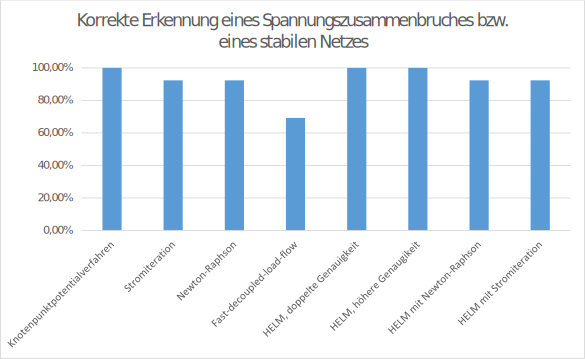
\includegraphics[scale=0.8]{pictures/convergence}
		\caption{Konvergenzverhalten der Berechnungsverfahren}
		\label{fig:convergence}
	\end{figure}
	
	Um die unterschiedlichen Berechnungsverfahren möglichst gut vergleichen zu können habe ich eine weitere Benutzeroberfläche in \emph{CalculationComparison} implementiert. Diese ermöglicht alle implementierten Berechnungsverfahren anhand einiger relativ zufällig gewählter Netze zu vergleichen bezüglich Genauigkeit, Konvergenzverhalten und Geschwindigkeit. Beginnen möchte ich hier mit \reffig{convergence}, welche die Anzahl der Netze darstellt, in welchen das jeweilige Verfahren korrekt konvergiert. In diesem Fall kommt es nicht zu der Situation einer Konvergenz zu einem instabilen Arbeitspunkt, daher ist nur die Information darüber ob das Verfahren konvergiert oder nicht relevant. Einige der Beispielnetze sind auch bewusst so gewählt, dass sich ein Spannungszusammenbruch ergibt. In diesen Fällen ist natürlich dann ein korrektes Konvergenzverhalten gegeben wenn das Verfahren nicht konvergiert und somit den Spannungszusammenbruch detektiert. Die Größe des Datentyps ist in \emph{HELM} mit höherer Genauigkeit dabei jeweils so konfiguriert, dass von der Genauigkeit her mit den iterativen Verfahren vergleichbare Ergebnisse erreicht werden. Exakt gleiche Ergebnisse sind natürlich nicht möglich, ein paar Verfahren konvergieren gar nicht für alle Testnetze korrekt. Allerdings konnte ich mit den standardmäßig angepassten Parametern vergleichbare Resultate bezüglich der Genauigkeit erreichen. Um dies mit \emph{HELM} zu erreichen ist es teilweise nötig einen Datentyp mit mehreren tausend Bit Genauigkeit zu wählen. Außerdem sei noch zu erwähnen, dass die Varianten \emph{HELM} mit \emph{Stromiteration} und \emph{HELM} mit \emph{Newton-Raphson} sich ein klein wenig von denen in \refsec{implementierung} unterscheiden. In diesem Fall wird immer zuerst \emph{HELM} mit 64 Bit zur Ermittlung der Startwerte ausgeführt und von diesen Werten aus das jeweilige iterative Verfahren gestartet. Somit stellen die beiden Verfahren in diesem Abschnitt nur einen Zwischenschritt der Verfahren in \refsec{implementierung} dar.
	
	\begin{figure}
		\centering
		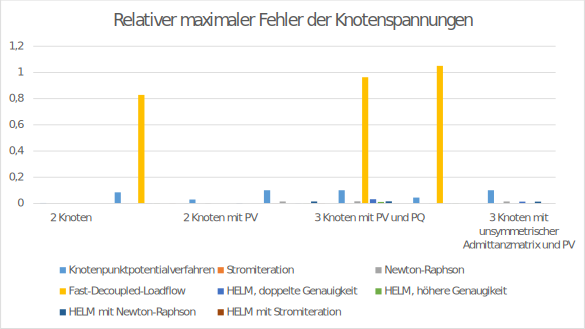
\includegraphics[scale=0.8]{pictures/precision_1}
		\caption{Genauigkeit der Berechnungsverfahren}
		\label{fig:precision_1}
	\end{figure}
	
	\begin{figure}
		\centering
		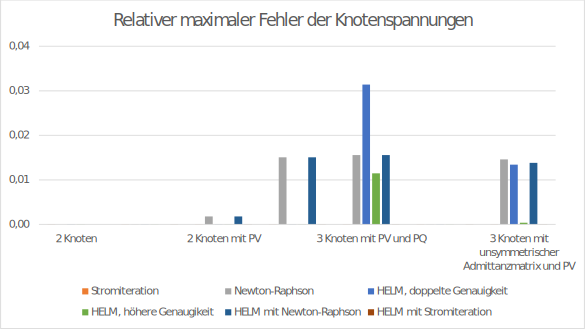
\includegraphics[scale=0.8]{pictures/precision_2}
		\caption{Genauigkeit der Berechnungsverfahren}
		\label{fig:precision_2}
	\end{figure}
	
	Als nächsten Aspekt gehe ich nun auf die Genauigkeit der Verfahren ein, welche durchaus variiert. Hierfür findet sich in \reffig{precision_1} und \reffig{precision_2} nur eine reduzierte Auswahl der Testnetzen von \reffig{convergence}, nämlich auf jene, bei denen alle Verfahren zumindest konvergieren. In \reffig{precision_1} zeigt sich allerdings, dass das \emph{Knotenpunktpotentialverfahren} und \emph{FDLF} teilweise trotzdem nicht wirklich brauchbare Ergebnisse liefern. In \reffig{precision_2} findet sich deswegen noch einmal der selbe Durchlauf, allerdings ohne die beiden zuletzt genannten Verfahren. In diesem Diagramm ist gut erkennbar, dass \emph{HELM} mit nur 64 Bit Rechengenauigkeit in manchen Fällen noch keine ausreichend exakten Ergebnisse ausgibt. Die anderen Verfahren hingegen zeigen ausreichend kleine und vergleichbare Fehler um einen Blick auf die Berechnungsdauer werfen zu können.
	
	\begin{figure}
		\centering
		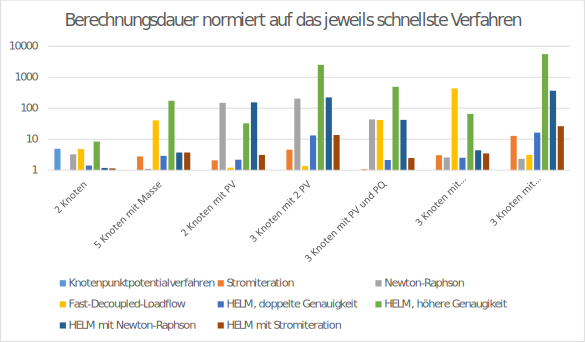
\includegraphics[scale=0.8]{pictures/duration_mean}
		\caption{durchschnittliche Berechnungsdauer der Verfahren}
		\label{fig:duration_mean}
	\end{figure}
	
	\begin{figure}
		\centering
		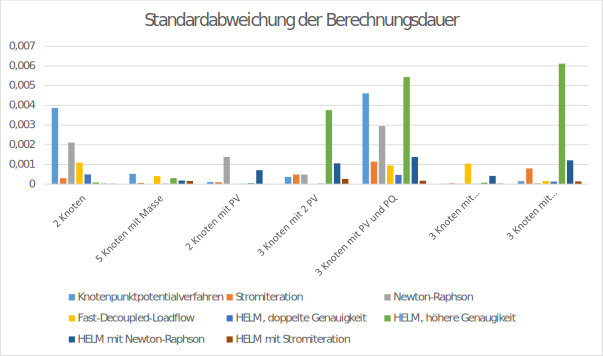
\includegraphics[scale=0.8]{pictures/duration_deviation}
		\caption{Standardabweichung der Berechnungsdauer der Verfahren}
		\label{fig:duration_deviation}
	\end{figure}
	
	Zu guter Letzt stellt sich noch die Frage der Berechnungsdauer, welche insbesondere bei größeren Netzen ein relevanter Aspekt wird. Hierbei erkennt man in \reffig{duration_mean} den Nachteil der höheren Rechengenauigkeit von \emph{HELM} mit einem genaueren Datentyp. Dementsprechend vermute ich vor allem akademische Anwendungsgebiete für \emph{HELM} mit beliebiger Genauigkeit. Der Vollständigkeit halber sind in \reffig{duration_deviation} noch die Schätzungen der Standardabweichungen angegeben welche deutlich zeigen, dass es sich in \reffig{duration_mean} um keine einzelnen Ausreißer handelt.
	
	\begin{figure}
		\centering
		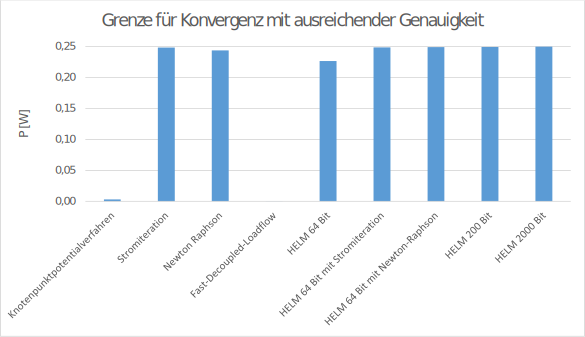
\includegraphics[scale=0.8]{pictures/convergence_border_1}
		\caption{Iterativ ermittelte Lastgrenze, bei der das Verfahren noch mit einer ausreichenden Genauigkeit konvergiert}
		\label{fig:convergence_border_1}
	\end{figure}
	
	\begin{figure}
		\centering
		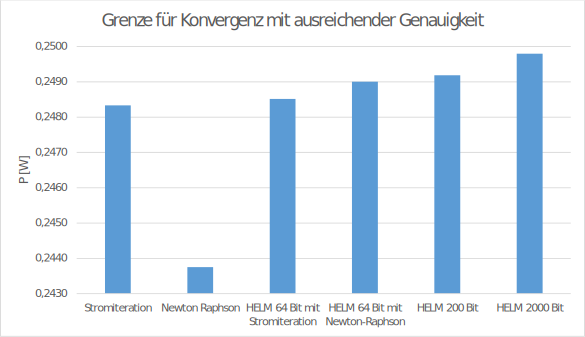
\includegraphics[scale=0.8]{pictures/convergence_border_2}
		\caption{Iterativ ermittelte Lastgrenze, bei der das Verfahren noch mit einer ausreichenden Genauigkeit konvergiert, reduziert um das \emph{Knotenpunktpotentialverfahren}, \emph{FDLF} und \emph{HELM} mit 64 Bit}
		\label{fig:convergence_border_2}
	\end{figure}
	
	\begin{figure}
		\centering
		\begin{circuitikz}	
	\draw (0, 0) node[above] {$U_1$} to [R=$Z$,o-o] (4, 0) node[above] {$U_2$};
	\draw[-stealth] (4, 0) --++ (0,-1);
	\draw (4.5, -1) node {$P$};
\end{circuitikz} 

		\caption{Netz zur Ermittlung der Konvergenzgrenze}
		\label{fig:two_node_net}
	\end{figure}
	
	\emph{HELM} ist aber ein durchaus interessanter Ansatz für Netze, welche nahe am Spannungszusammenbruch betrieben bzw. berechnet werden. Um dieses mögliche Einsatzgebiet zu überprüfen habe ich in dem kleinen Netz in \reffig{two_node_net} mit nur einer Einpeisung, einer Last und einer Verbindung dazwischen sukzessive die Last erhöht bis das jeweilige Berechnungsverfahren einen Spannungszusammenbruch detektierte bzw. keine ausreichende Genauigkeit mehr gegeben war. Aufgrund der einfachen Struktur des Netzes lässt sich zudem rechnerisch zeigen, dass die tatsächliche Stabilitätsgrenze bei $P = \SI{0.25}{\watt}$ liegt. In \reffig{convergence_border_1} und \reffig{convergence_border_2} zeigen sich die besseren Eigenschaften von \emph{HELM}, verglichen mit den klassischen iterativen Verfahren, bei der Berechnung eines Netzes nahe am Spannungszusammenbruch.
	
	\begin{figure}
		\centering
		\includegraphics[scale=0.55]{pictures/complete_powernet_modified}
		\caption{Testnetz zur Überprüfung der Modellierung}
		\label{fig:powernet_complete}
	\end{figure}
	
	Zu guter Letzt möchte ich noch erwähnen, dass ich für einige Testnetze, unter anderem für \reffig{powernet_complete}, die Ergebnisse der Lastflussberechnung mit \emph{PSS SINCAL} verfiziert habe um Fehler in der Modellierung der Netzelemente ausschließen zu können.
	
	\section{Fazit}
	\emph{HELM} verspricht theoretisch die idealen Eigenschaften für ein Verfahren zur Lastflussberechnung. Aufgrund numerischer Einschränkungen, bedingt durch eine begrenzte Rechengenauigkeit, ergibt sich allerdings ein durchaus relevanter Nachteil: Man muss für \emph{HELM}, in Reinform, abwägen zwischen Genauigkeit und Rechenzeit. Die Verschlechterung der Performance führt dabei zu Rechenzeiten welche um Größenordnungen schlechter sind als jene für die klassischen Verfahren wie die \emph{Stromiteration} oder \emph{Newton-Raphson}. Wenn man allerdings \emph{HELM} mit nur 64 Bit mit einem iterativen Verfahren verbindet ist es möglich die Vorteile beider Verfahren zu kombinieren.
	
	Schlussendlich ist also \emph{HELM} kein Allheilmittel, es stellt allerdings eine durchaus nützliche Alternative dar. Welches Berechnungsverfahren nun das ideale ist hängt sehr stark von der jeweiligen Situation ab. Mit \emph{HELM} hat man dabei allerdings eine weitere Option, welche sich insbesonders für Systeme nahe am Spannungszusammenbruch anbietet.
	
	\begin{thebibliography}{1}
		\bibitem{helmIEEE}
			A.~Trias, \emph{The Holomorphic Embedding Load Flow Method}, IEEE PES General Meeting, July 2012
		\bibitem{helmPV}
			M.~K.~Subramanian, Y.~Feng, D.~Tylavsky, \emph{PV Bus Modeling in a Holomorphically Embedded Power-Flow Formulation}, 978-1-4799-1255-1/13, IEEE, 2013
		\bibitem{helmPatentApr2009} 
			A.~Trias, \emph{System and Method for Monitoring and Managing Electrical Power Transmission and Distribution Networks}, US Patent 7,519,506 B2, April 2009
		\bibitem{helmPatentSept2009} 
			A.~Trias, \emph{System and Method for Monitoring and Managing Electrical Power Transmission and Distribution Networks}, US Patent US 2009/0228154 A1, September 2009
			
		\bibitem{epsilonWynn}
			P.~Wynn, \emph{The Epsilon Algorithm and Operational Formulas of Numerical Analysis}, June 1960

	\end{thebibliography}

\end{document}